\documentclass[a4paper, 12pt]{article}

\usepackage[italian]{babel}
\usepackage{graphicx}
\usepackage{float}

\linespread{1.5}



\title{Sintesi di Composti d'interesse Medico per il Trattamento del Morbo d'Alzheimer}
\author{
	Relatore: Annamaria DeAgostino
	\and
	Candidato: Lorenzo Castellino
}
\date{Anno Accademico 2018-2019}

\begin{document}
\pagenumbering{gobble}
\maketitle
\setcounter{page}{0}
\newpage
\tableofcontents
\newpage
\pagenumbering{arabic}

\section{Introduzione al Morbo d'Alzheimer}
La malattia di Alzheimer-Perusini, nota più comunemente come morbo d'Alzheimer (AD), è una tra le forme più diffuse al mondo di demenza senile. Dal punto di vista medico la patologia è definita come "disturbo neurocognitivo maggiore o lieve dovuto a malattia di Alzheimer".\cite{american_psychiatric_association_diagnostic_2013}
I sintomi associati sono differenti da individuo ad individuo, in generale nei pazienti riconosciuti si sono osservate:
\begin{enumerate}
	\item Perdita di memoria a breve termine.
	\item Difficoltà a concentrarsi, organizzarsi e di pianificazione.
	\item Difficoltà a seguire e/o formulare discorsi di senso compiuto.
	\item Difficoltà a giudicare distanze e spazi.
	\item Perdita di orientamento spaziale e temporale.
	\item Cambi repentini dell'umore.
	\item Allucinazioni visive.
\end{enumerate}
La demenza è una patologia di tipo progressivo, ovvero si ha un peggiormento dei sintomi col passare del tempo. La velocità di tale processo varia da persona a persona, tendenzialmente l'aspettativa media di vita successiva alla diagnosi della condizione va dai 3 ai 10 anni. \cite{todd_survival_2013}

\subsection{L'Importanza della Ricerca}
L'incidenza dell'AD è in aumento tanto da individuare la ricerca di una cura come una delle sfide per il nuovo millenio: stando al World Alzheimer Report del 2018, stilato dall'Alzheimer's Disease International ovvero l'associazione internazionale per la lotta all'Alzheimer in stretta collaborazione con la World Health Organization, si stima che nel mondo circa 50 milioni di persone siano affette da demenza. Ciò si traduce in una spesa annua per il trattamento dei malati che rasenta il miliardo di dollari.

Con l'aumento dell'aspettativa media di vita si prevede che nel 2050 il numero di casi sarà il triplo di quello odierno e si prospetta una spesa doppia rispetto a quella attuale.\cite{noauthor_world_2018}

Stando a queste previsioni 1'individuo su 85 nel 2050 sarà affetto da demenza.

L'individuazione delle cause che portano al presentarsi dell'AD è uno dei punti salienti della ricerca in campo medico e biochimico, sono state portate avanti molte ipotesi a riguardo. Al momento una delle tesi più avvalorate e studiate è quella della formazione di aggregati proteici nel liquido cerebrospinale.

\subsection{$\beta$-Amiloidi e Placche Amiloidiche}
\label{sec:ab}
Con il termine $\beta$-amiloide (A$\beta$) si indica un frammento proteico insolubile non ramificato, il nome è dovuto al fatto che al momento della scoperta, viste le sue proprietà si pensò in ad una similitudine con le molecole d'amido benchè dal punto di vista della composizione chimica non ci siano particolari somiglianze.\cite{lennarz_encyclopedia_2004}

L'origine di queste strutture è legata all'azione congiunta di tre enizmi ($\alpha$-secretasi,$\beta$-secretasi e $\gamma$-secretasi) su di un substrato proteico noto come APP (Amyloid Precursor Protein). L'APP è una proteina trans-membrana di modeste dimensioni (circa 700 residui), viene trasportata lungo l'assone delle cellule neuronali e il suo accumulo è focalizzato nei siti presinaptici. Il suo rilascio è regolato dall'attività elettrica cerebrale, si suppone infatti che abbia un ruolo fondamentale nella regolazione dell'eccitabilità neuronale.\cite{mattson_cellular_1997}
La porzione che interessa la formazione di A$\beta$ è situata nel dominio extracellulare dell'APP. Come si può osservare nella Figura \ref{fig:app} i tre enzimi sopracitati agiscono in punti ben definiti e tra loro differenti della proteina; in particolare si osservi come l'azione dell'$\alpha$-secretasi non porti alla formazione del frammento $\beta$A mentre l'azione dell'enzima $\beta$ in congiunzione all'enzima $\gamma$ generi la particolare sequenza.\cite{goedert_century_2006}

\begin{figure}[H]
	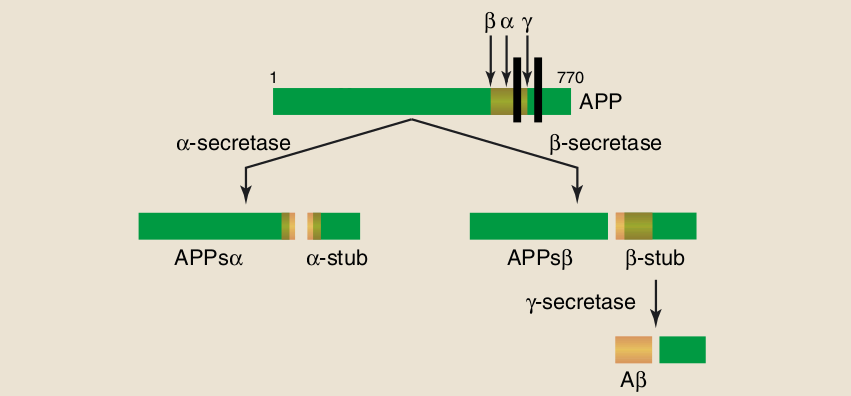
\includegraphics[width=\linewidth]{immagini/APP.png}
	\caption{Azione degli enzimi $\alpha$/$\beta$/$\gamma$-secretasi sul substrato APP.}
	\label{fig:app}
\end{figure}

I frammenti prodotti sono di due varietà che si differenziano per il numero di residui in essi contenuti, ecco quindi che possiamo distinguere i A$\beta$-40 e i A$\beta$-42 rispettivamente formati da 40 e 42 amminoacidi. Il rapporto tra le quantità prodotte delle due forme é di particolare importanza in quanto la $\beta$A-42 tende a formare oligomeri e fibrille più facilmente rispetto all’$\beta$A-40 molto probabilmente vista la minore solubilità data dai due residui idrofobici in più.\cite{kepp_bioinorganic_2012, irvine_protein_2008}

La produzione di $\beta$ in piccole quantità é un processo normale; delle funzioni osservate citiamo: \cite{brothers_physiological_2018}

\begin{enumerate}
	\item Funzione antibatterica, antifunginea e antivirale.
	\item Soppressione tumorale.
	\item Meccanismo di riparazione di falle nella barriera emato-encefalica (azione simile alle piastrine nel sangue).
	\item Regolazione dell'attività sinaptica.
\end{enumerate}

Malgrado i benefici per l'organismo una sovrapproduzione di A$\beta$ o una sproporzione verso la forma contenente 42 residui associata ad uno smalitmento non efficacie sembra essere una causa sufficiente per lo sviluppo precoce del Morbo d’Alzheimer. \cite{irvine_protein_2008}
La demolizione avviene sia direttamente nel cervello, come abbiamo infatti visto l'$\alpha$-secretasi effettivamente rende innocui i frammenti amiloidici scindendoli in due porzioni inerti; ma una gran parte di essa è delegata ad enzimi demolitori presenti nel fegato. La diffusione del frammento proteico insolubile è regolata dal recettore proteico LRP1 il cui processo di endocitosi è contrastato dall'azione del recettore antagonista RAGE (Figura \ref{fig:bbb}).\cite{lillis_beyond_2005, dries_extracting_2012}

\begin{figure}[H]
	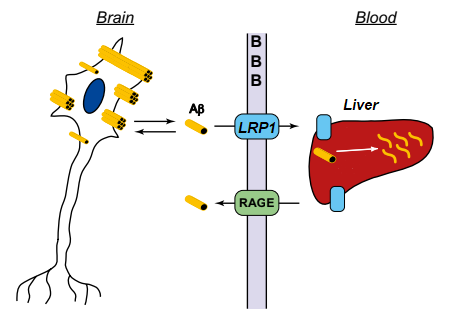
\includegraphics[width=\linewidth]{immagini/bbb.png}
	\caption{Fenomeno di migrazione dei A$\beta$ attraverso la barriera emato-encefalica (BBB) verso il fegato ed effetto inverso legato al recettore RAGE).}
	\label{fig:bbb}
\end{figure}

All'aumento della concentrazione di A$\beta$ nel liquido cerebrospinale è infatti associata la tendenza alla formazione di aggregati proteici più grandi ed insolubili detti comunemente "placche" o "fibrille".
L'accumulo di queste altera la chimica delle sinapsi, rallentando la trasmissione tra neuroni fino al punto di impedirla, causando così infine la morte della cellula.

Altre evidenze sperimentali mostrano come l’organismo, a causa di invecchiamento o condizioni di stress, come ad esempio la mancanza di sonno, risulta meno efficiente nella loro demolizione, amplificando gli effetti di accumulo nel liquido cerebrospinale.

Gli scarsi risultati ottenuti seguendo la via della neurotossicità diretta dei A$\beta$ ha portato alla teorizzazione e in seguito all’osservazione di concentrazioni anormali di ioni metallici in pazienti affetti dall'AD. I metalli presi in esame sono Ferro, Rame e Zinco le cui concentrazioni, superato il valore di circa 10\textsuperscript{-7}  M diventano rilevanti per quanto riguarda la possibilità di essere complessati dai A$\beta$ causando una tossicità diretta o fungendo come centri iniziatori di polimerizzazione per le fibrille amiloidiche.\cite{kepp_bioinorganic_2012}

\section{Strategie d'Intervento}
Visto il complesso sistema che regola la comparsa dei A$\beta$ vien da se che anche i metodi per cercare di limitarne la presenza o gli effetti sull'organismo saranno altrettanto variegati.

Le metodologie d'intervento studiate nel panorama della ricerca biomedica sono tra le più disparate, limitandoci solo a tecniche che agiscono direttamente sui A$\beta$ o sui loro effetti sull'organismo possiamo citare:\cite{kumar_review_2015}
\begin{enumerate}
	\item Mitigazione del trasporto dei A$\beta$ agendo sull'attività recettori LRP1 e RAGE.
	\item Modulazione degli enzimi responsabili della formazione di A$\beta$, in particolare modulando la demolizione tramite l'$\alpha$-secretasi o inibendo la produzione per mezzo della $\beta$-secretasi.
	\item Limitazione dell'aggregazione dei A$\beta$ in oligomeri e placche.
	\item Vaccinazione con oligomeri di A$\beta$, l'intento è quello di stimolare una risposta immunitaria all'accumularsi degli aggregati amiloidici.
	\item Modulazione della neurotrasmissione in modo da limitare l'effetto d'inibizione delle sinapsi.
	\item Mitigazione degli effetti da stress ossidativo.
\end{enumerate}

Nella seguente trattazione ci limiteremo a presentarne alcuni con esempi di composti potenzialmente interessanti dal punto di vista farmacologico soffermandoci infine in maniera più estesa su di un possibile processo di sintesi per ognuno di essi.
La discussione verterà in particolare attorno a due composti la cui azione potrebbe limitare e rallentare la neurodegenerazione nelle Sezioni \ref{sec:resv} e \ref{sec:curc}, per poi affrontare invece una possibile tecnica mirata a prevenire il presentarsi dell'AD nella Sezione \ref{sec:byp}

\section{Resveratolo}
\label{sec:resv}

\section{Curcumina}
\label{sec:curc}

\section{Leganti Bipiridinici}
\label{sec:byp}
Andiamo ora a considerare una classe di composti la cui azione non è legata alla regolazione dell'attività ormonale ma ad una mitigazione del fenomeno d'aggregazione in placche dei A$\beta$. Come presentato nella Sezione \ref{sec:ab} uno dei meccanismi di aggregazione considerati alla base della formazione degli agglomerati proteici neurotossici prevede che il formarsi di un complesso tra metalli in concentrazioni sopra la norma nel liquido cerebrospinale e i A$\beta$ stessi.

L'idea alla base di un trattamento agente su questo meccanismo prevede una diminuzione dei metalli biodisponibili attraverso una chelazione degli stessi per mezzo di leganti organici.

\subsection{Le Molecole}
Per progettare una molecola in grado di svolgere il compito appena descritto occorrerà che questa soddisfi alcuni criteri:
\begin{enumerate}
	\item Capacità di complessare il metallo d'interesse.
	\item Costanti d'equilibrio elevate per quanto riguarda la forma complessata.
	\item Buona solubilità in ambiente acquoso, in modo da permettere la diffusione del composto all'interno del corpo.
	\item Buona permeabilità della barriera emato-encefalica, un composto che non soddisfi questo criterio avrà difficoltà ad essere trasferito nel liquido cerebrospinale.
\end{enumerate}
Una classe di composti le cui propietà soddisfano i criteri appena presentati è quella dei composti Bipiridinici (Figura \ref{fig:bpy}).
Questi presentano una chelazione rapida, ovvero con k\textsubscript{f} nei confronti dei metalli d'interesse (Cu(II) e Zn(II)) di circa 7.0, grazie alla chelazione dell'atomo metallico da parte degli atomi d'azoto nei due eterocicli. Inoltre la solubilità in medium acquosi è relativamente buona, stiamo parlando di circa 5,9 mg/mL; infine le dimensioni ridotte permettono una buona diffusione nel sistema nervoso permeando attravero la barriera emato-encefalica con discreta facilità (i valori di permeabilità possono essere stimati attraverso le regole empiriche di Lipinski o attraverso test in vitro\cite{di_high_2003}).
\begin{figure}[H]
	\centering
	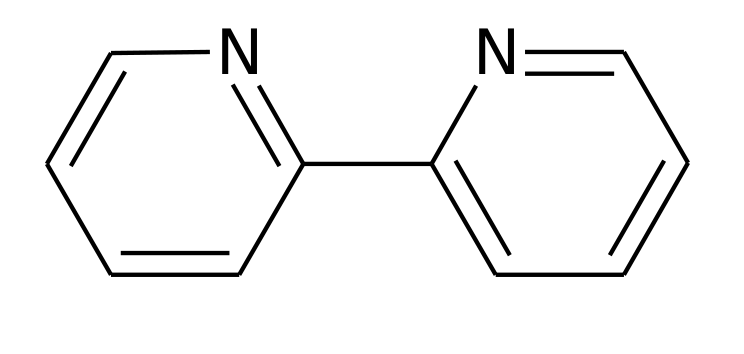
\includegraphics[width=.5\linewidth]{immagini/bpy.png}
	\caption{Un generico composto appartenente alla classe delle Bipiridine.}
	\label{fig:bpy}
\end{figure}
Lo scheletro bipiridinico ben si presta ad un approccio razionale nella sinstesi di composti interessanti dal punto di vista biomedico.
L'introduzione di gruppi dimetilamminici favorisce un'interazione con i A$\beta$ e per la sua influenza sul legame metallico come suggerito da alcune evidenze sperimentali. Similmente l'uso di un sostituente metilico permette un megliore effetto elettrodonatore da parte egli eteroatomi nei cicli e un controllo sterico sui possibili orientamenti con cui la molecola bipiridinica può interagire con il metallo. \cite{derrick_importance_2016,savelieff_ongoing_2014}




\newpage


\bibliographystyle{acm}
\bibliography{biblio.bib}
\end{document}
